\chapter{Capturas de pantalla}
La finalidad de este ap�ndice es ilustrar el resultado real de la aplicaci�n tras su implementaci�n mediante capturas de la mayor�a de sus interfaces y procesos.
\begin{figure}[htbp]
    \centering
    \subfigure[Formulario de inicio de sesi�n]{
   	 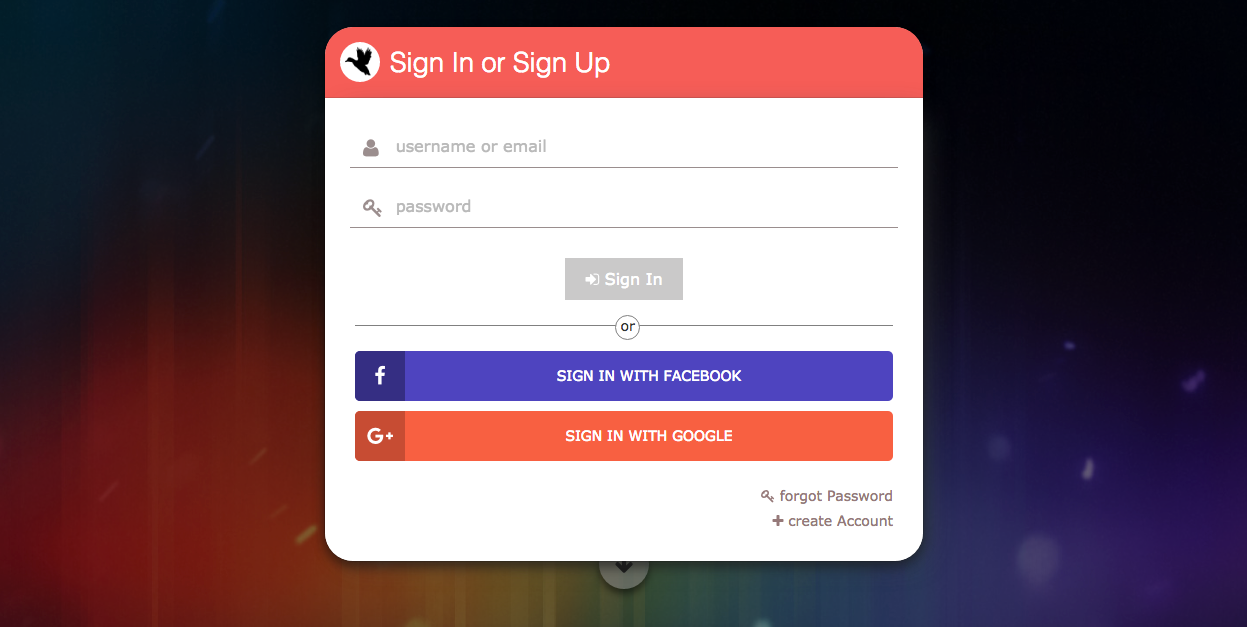
\includegraphics[width=0.7\textwidth]{sign-in-form.png}
    	\label{fig:signInReal}
    }
    \subfigure[Formulario de registro]{
    	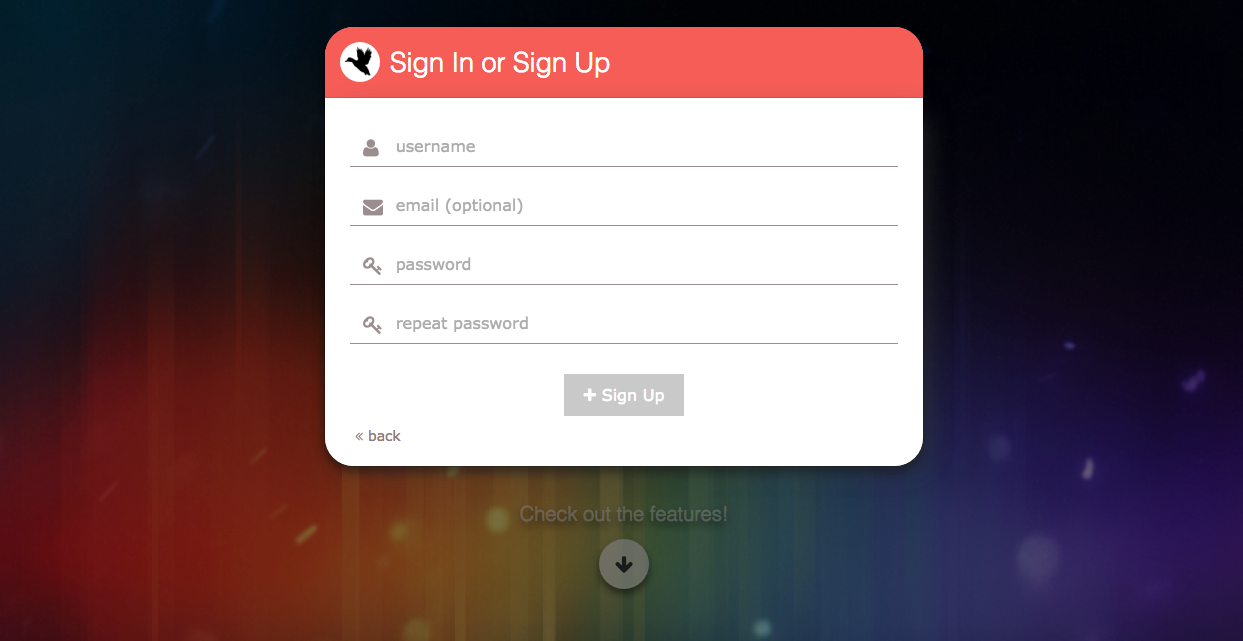
\includegraphics[width=0.7\textwidth]{sign-up-form.png}
	 \label{fig:signUpReal}
    }
    \caption{Formularios de registro en P�gina de inicio}
    \label{fig:signFormsReal}
\end{figure}

\begin{figure}[htpb]
	\centering
	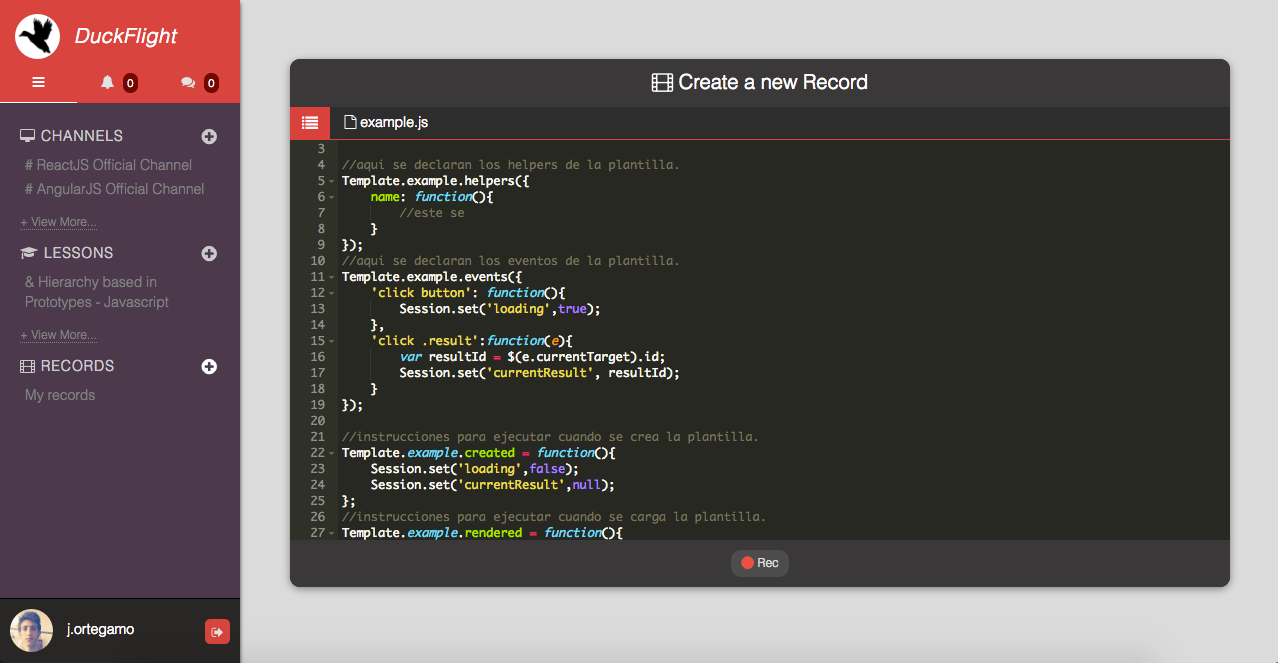
\includegraphics[width=0.75\textwidth]{recorder.png}
	\caption{Grabador}
	\label{fig:recorder}
\end{figure}
\begin{figure}[htpb]
	\centering
	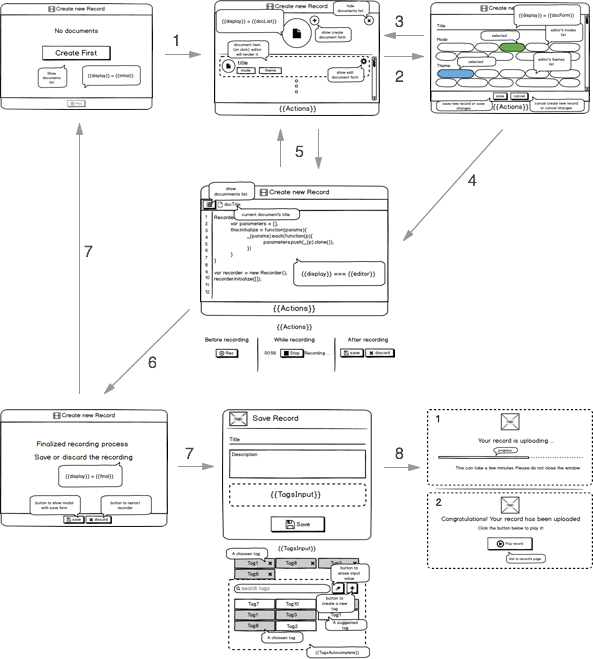
\includegraphics[scale=0.4]{recorderFlow.png}
	\label{fig:grabacionFlujo}
	\caption{Flujo de plantillas del grabador}
\end{figure}

\begin{figure}[htpb]
	\centering
	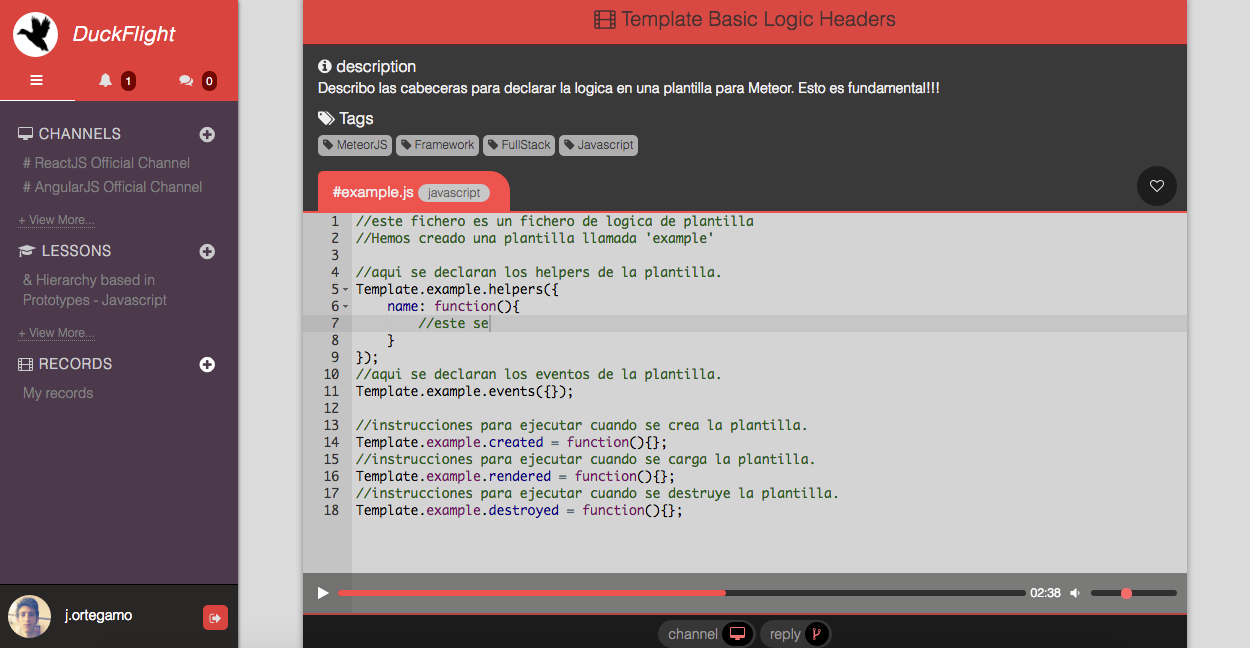
\includegraphics[width=0.8\textwidth]{record-player.png}
	\caption{Reproductor}
	\label{fig:recordPlayerPage}
\end{figure}

\begin{figure}[htpb]
	\centering
	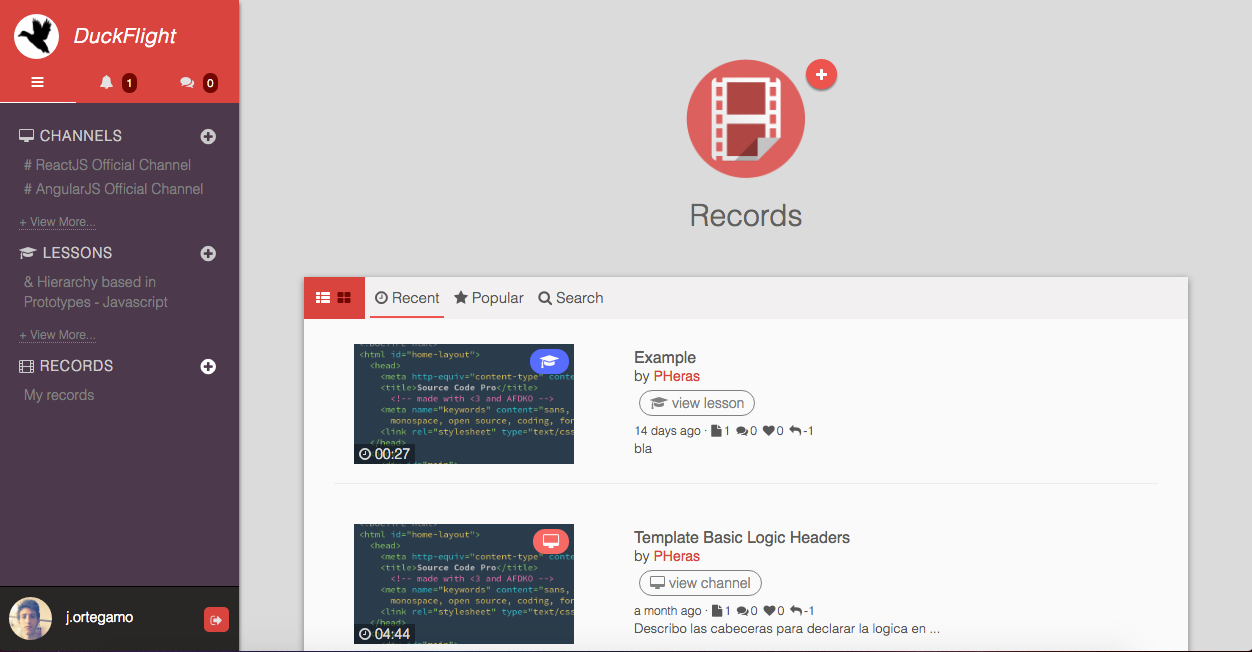
\includegraphics[width=0.8\textwidth]{records.png}
	\caption{Lista de grabaciones}
	\label{fig:records}
\end{figure}

\begin{figure}[htpb]
	\centering
	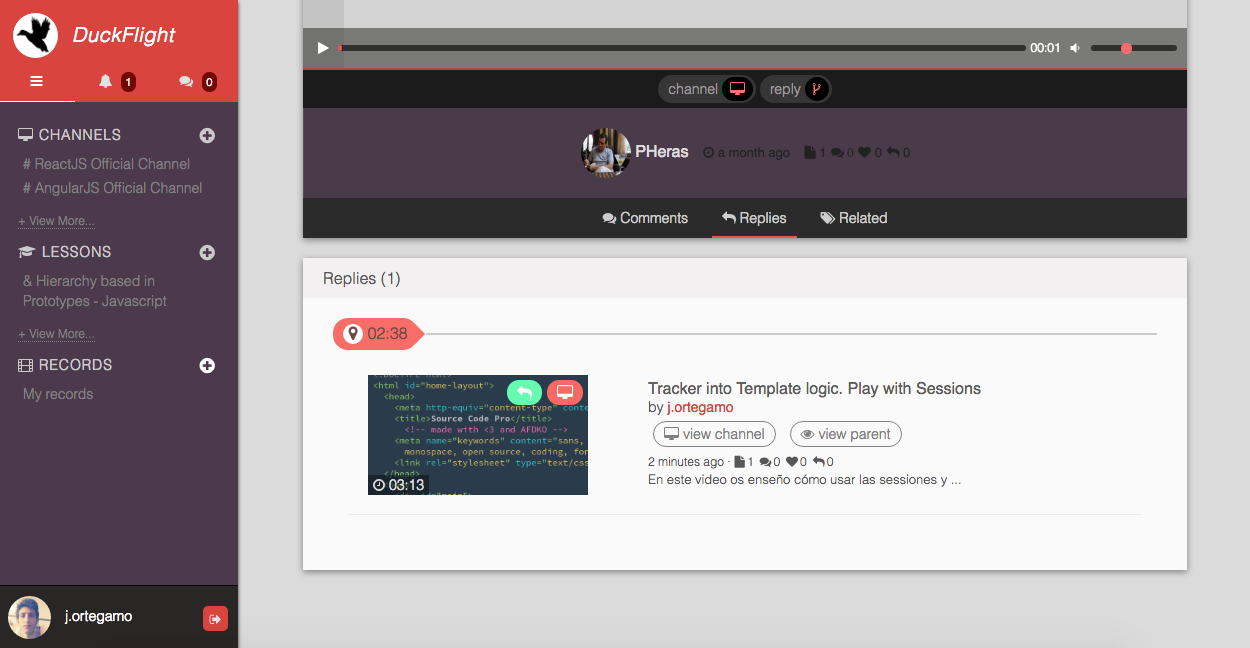
\includegraphics[width=0.8\textwidth]{replies-tab.png}
	\caption{Timeline de respuestas}
	\label{fig:replies-tab}
\end{figure}

\begin{figure}[htpb]
	\centering
	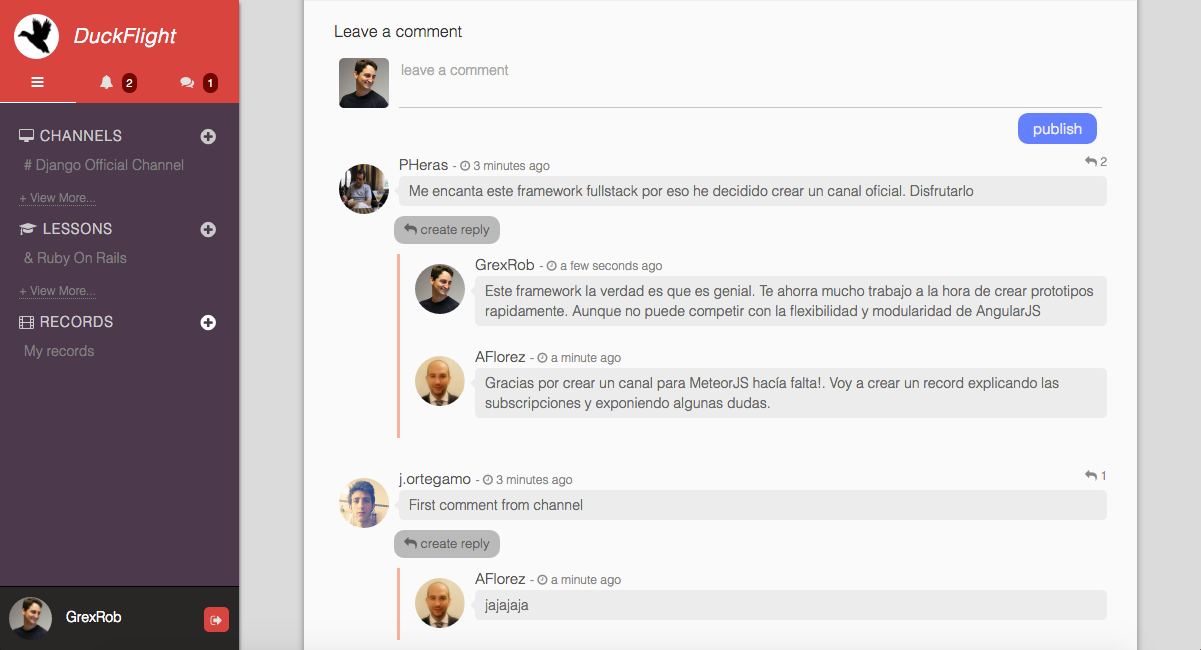
\includegraphics[width=0.8\textwidth]{comments-module.png}
	\caption{Espacio para comentarios}
	\label{fig:comments-module}
\end{figure}


\begin{figure}[htpb]
	\centering
	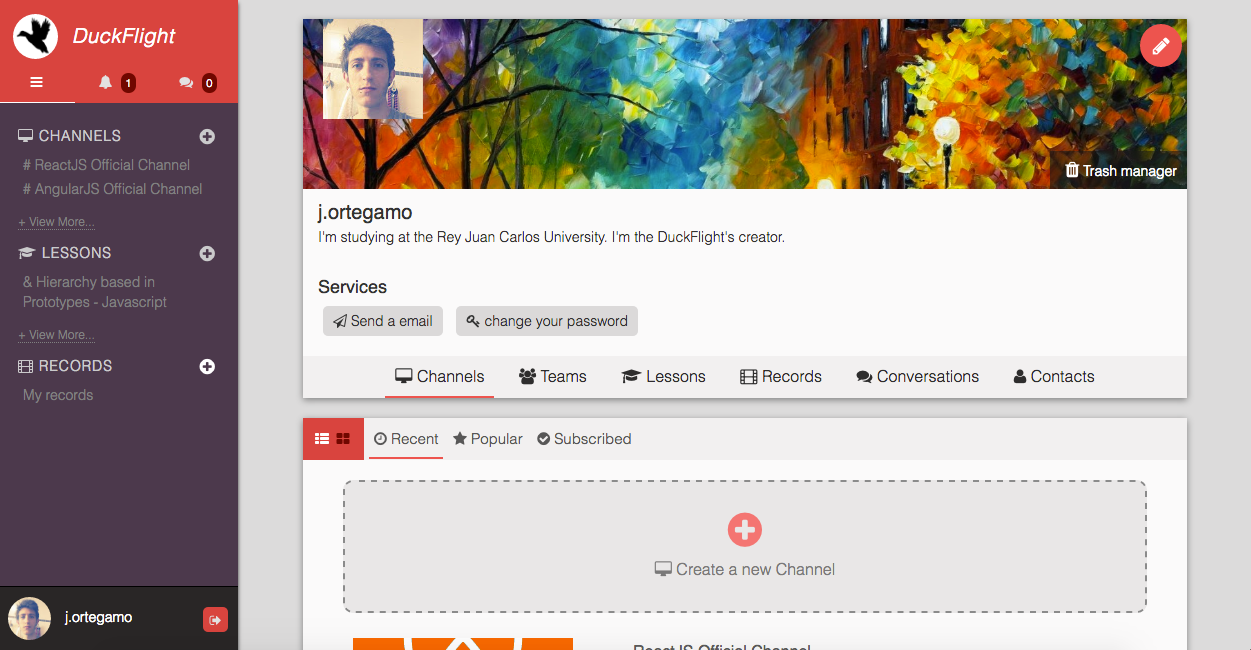
\includegraphics[width=0.8\textwidth]{profile-page.png}
	\caption{P�gina del perfil}
	\label{fig:profile-page}
\end{figure}

\begin{figure}[htpb]
	\centering
	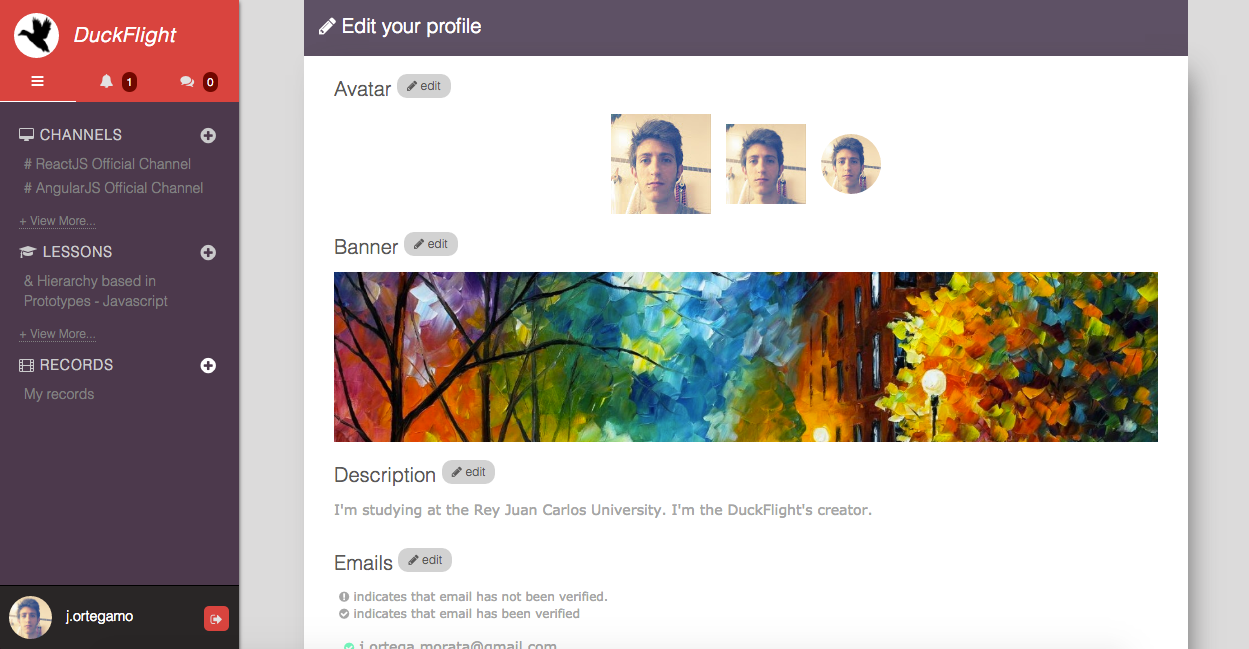
\includegraphics[width=0.8\textwidth]{profile-edit.png}
	\caption{P�gina de edici�n del perfil}
	\label{fig:profile-edit}
\end{figure}

\begin{figure}[htpb]
	\centering
	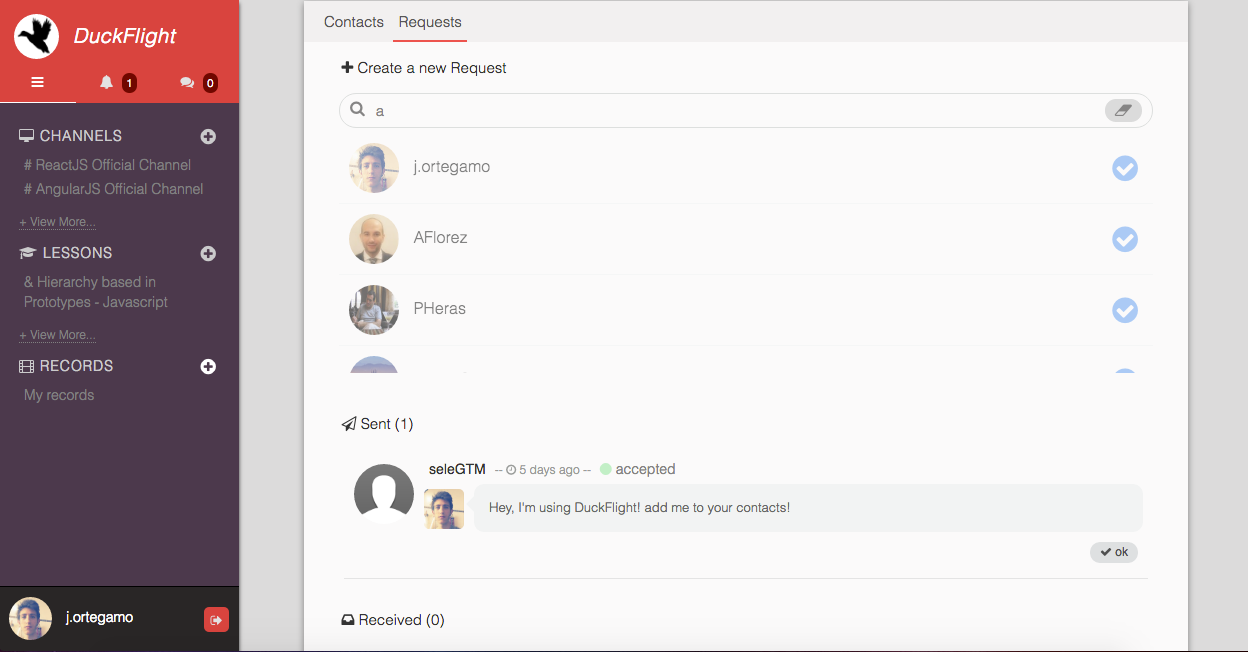
\includegraphics[width=0.8\textwidth]{contacts-requests.png}
	\caption{Espacio para peticiones de contacto}
	\label{fig:contacts-requests}
\end{figure}

\begin{figure}[htpb]
	\centering
	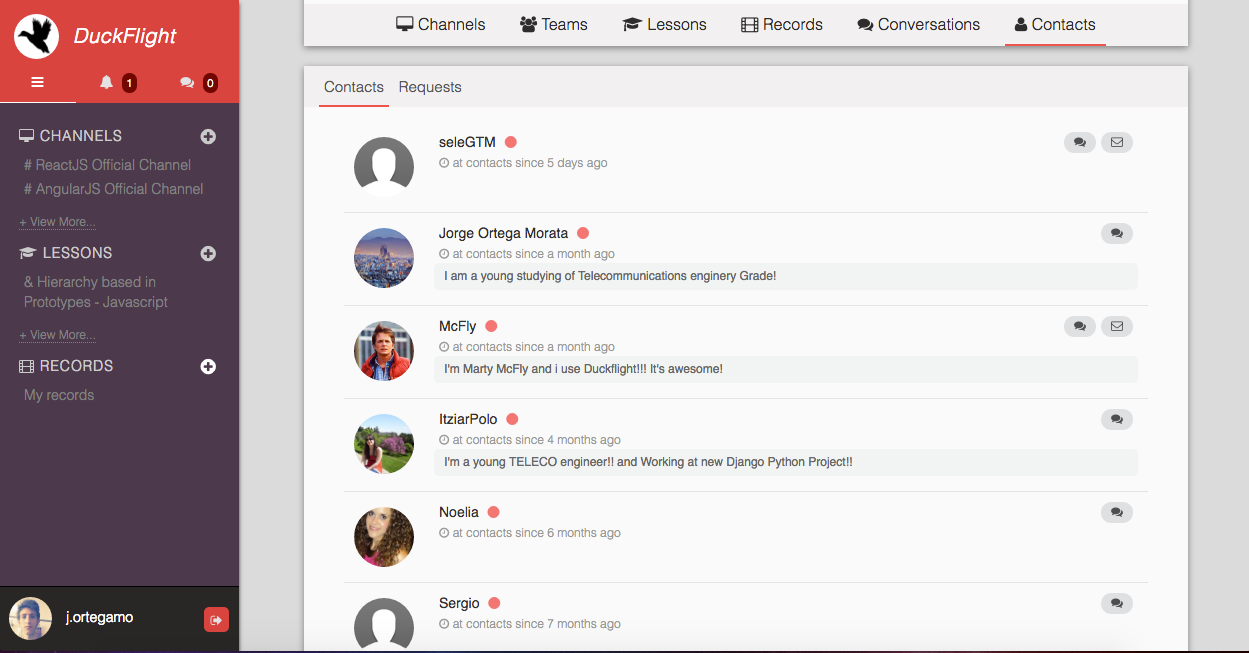
\includegraphics[width=0.8\textwidth]{contacts.png}
	\caption{Lista de contactos}
	\label{fig:contacts-tab}
\end{figure}

\begin{figure}[htpb]
	\centering
	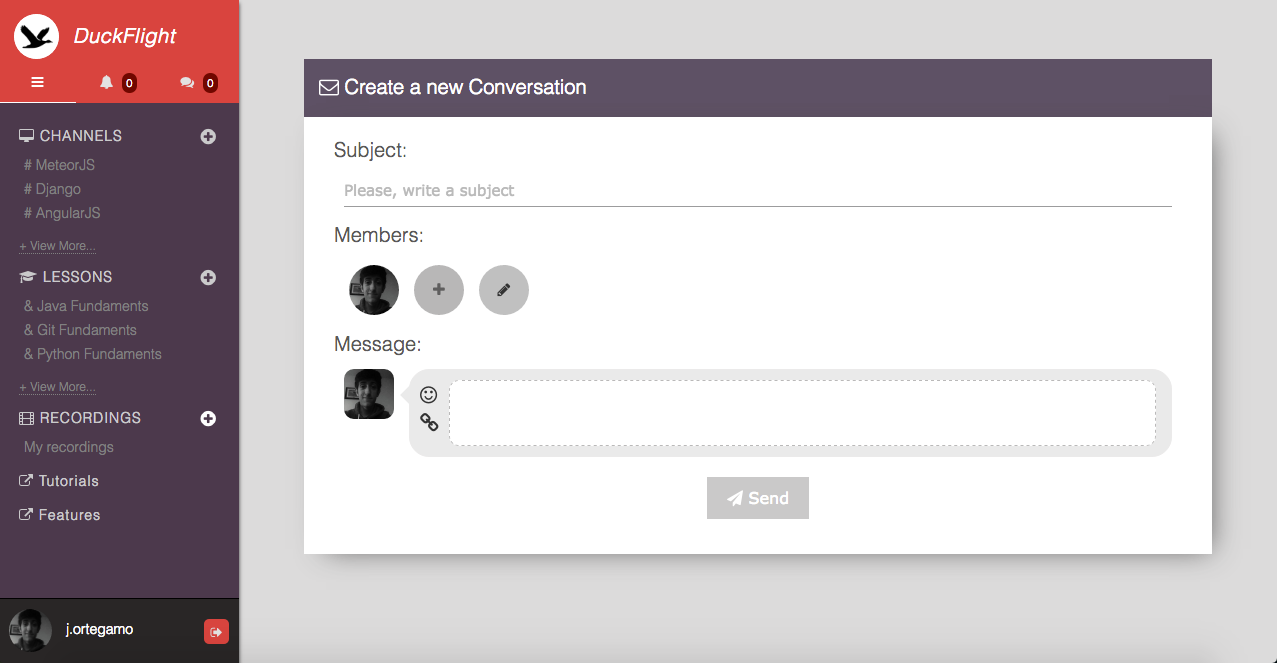
\includegraphics[width=0.8\textwidth]{conversation-create.png}
	\caption{Formulario de creaci�n de una conversaci�n}
	\label{fig:conversation-create}
\end{figure}

\begin{figure}[htpb]
	\centering
	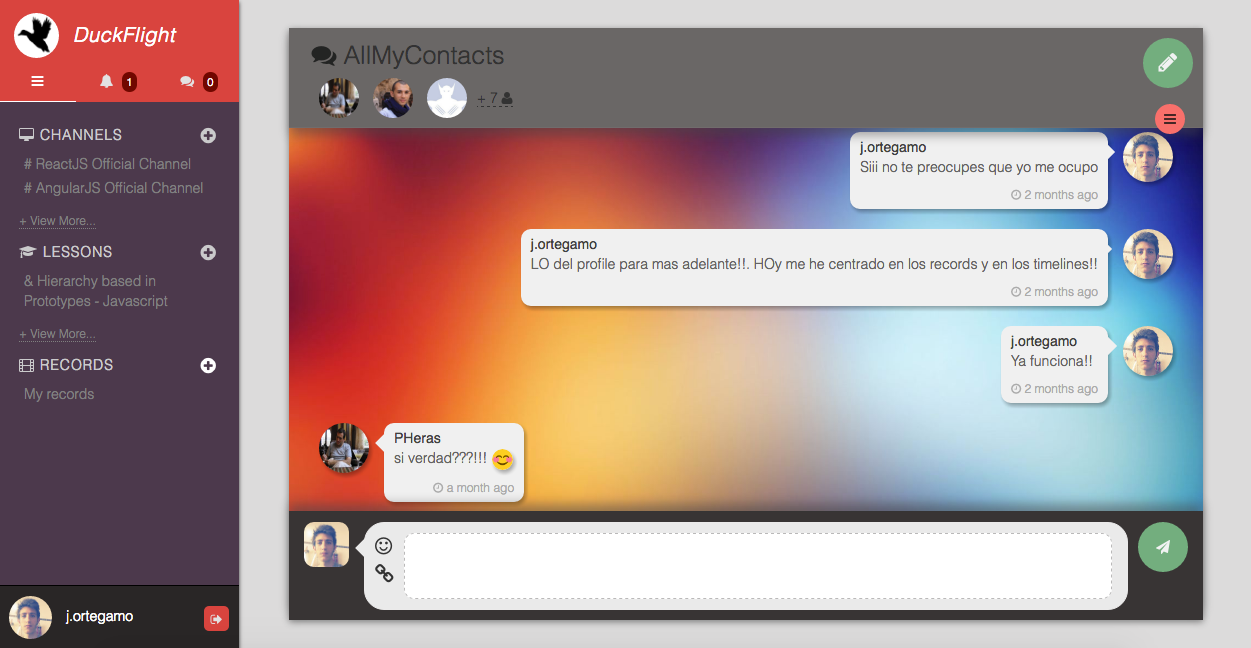
\includegraphics[width=0.8\textwidth]{conversation-page.png}
	\caption{P�gina de una conversaci�n}
	\label{fig:conversation-page}
\end{figure}

\begin{figure}[htpb]
	\centering
	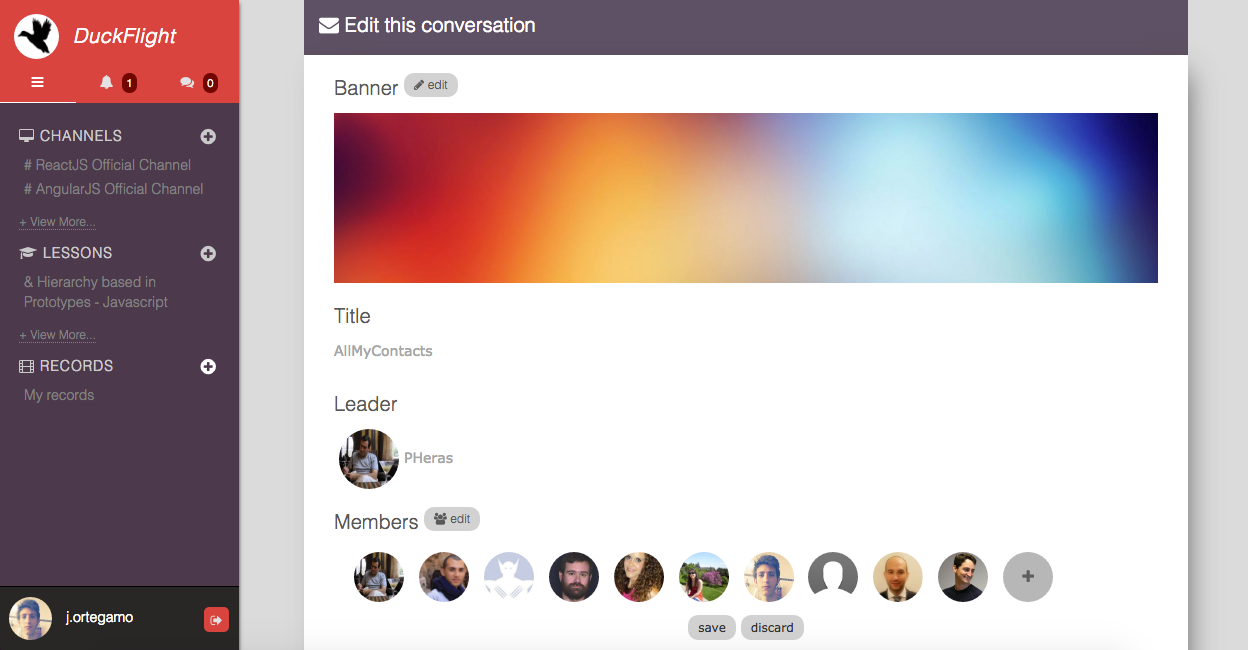
\includegraphics[width=0.8\textwidth]{conversation-edit.png}
	\caption{Formulario de edici�n de una conversaci�n}
	\label{fig:conversation-edit}
\end{figure}





\begin{figure}[htpb]
	\centering
	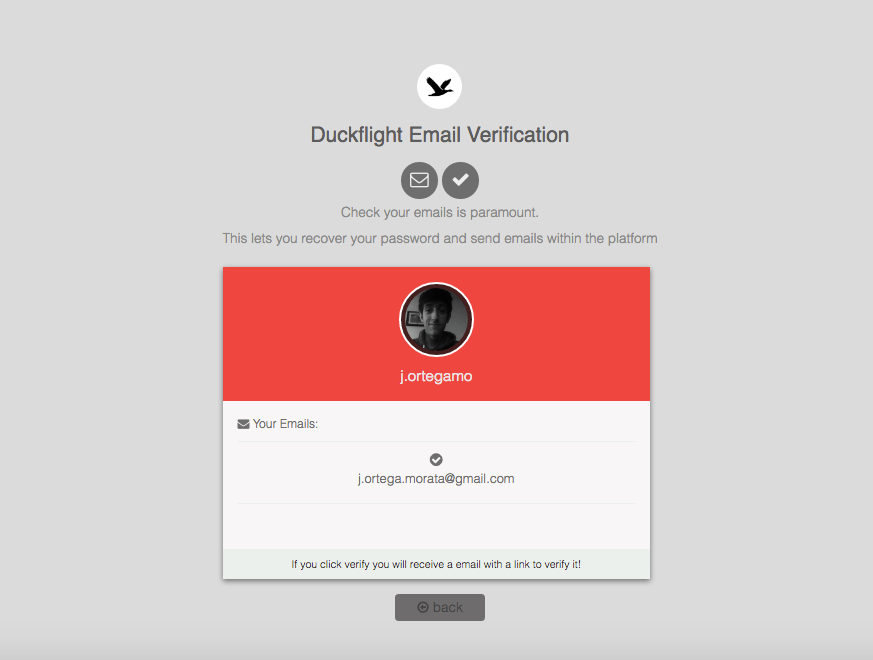
\includegraphics[width=0.8\textwidth]{verifications.png}
	\caption{Proceso de verificaci�n de emails}
	\label{fig:verifications-page}
\end{figure}

\begin{figure}[htpb]
	\centering
	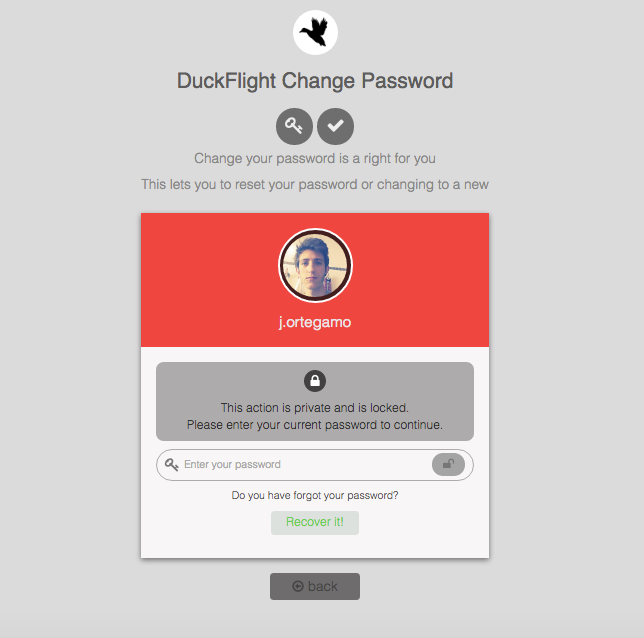
\includegraphics[width=0.8\textwidth]{change-password.png}
	\caption{Proceso de cambio de contrase�a}
	\label{fig:change-password}
\end{figure}

\begin{figure}[htpb]
	\centering
	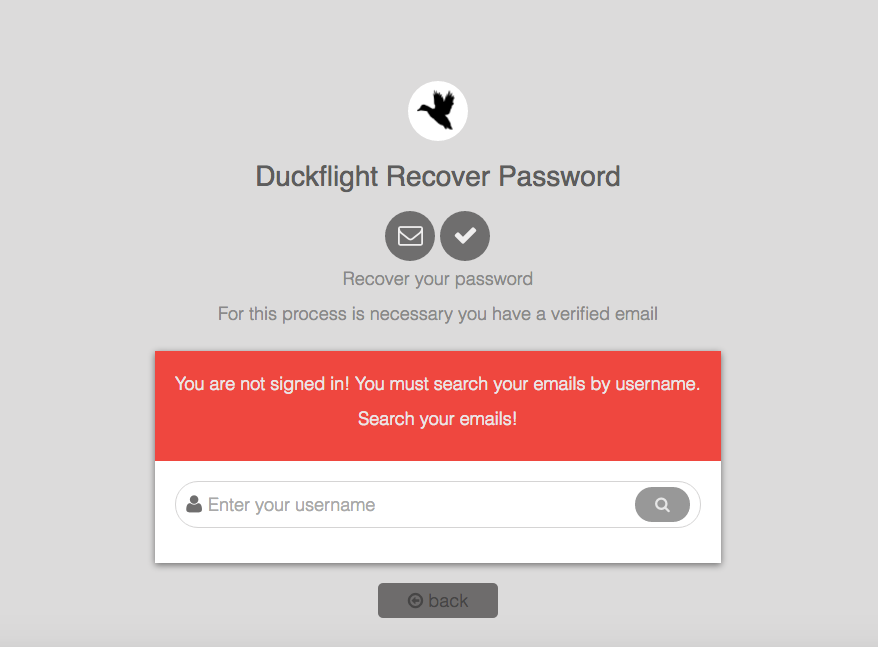
\includegraphics[width=0.8\textwidth]{forgot-password-form.png}
	\caption{Proceso de recuperaci�n de contrase�a}
	\label{fig:forgot-password-form}
\end{figure}

\begin{figure}[htpb]
	\centering
	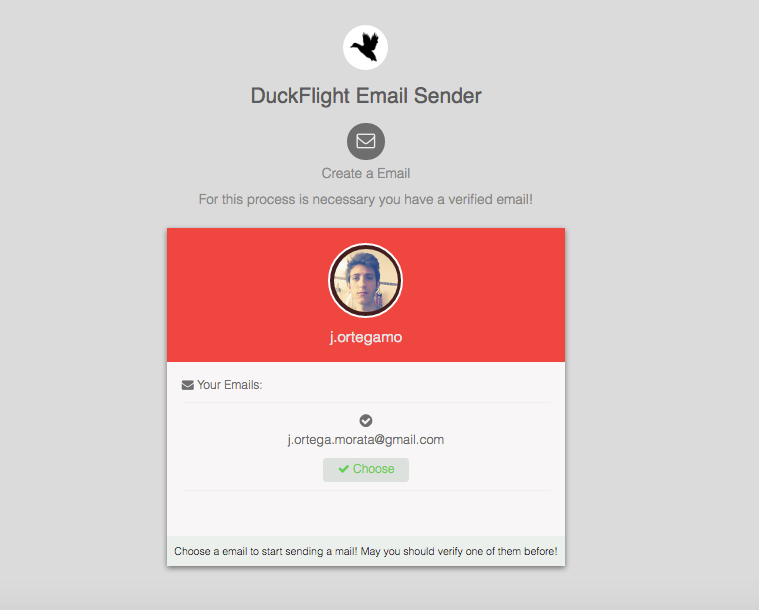
\includegraphics[width=0.8\textwidth]{email-sender.png}
	\caption{P�gina de selecci�n de email}
	\label{fig:email-sender}
\end{figure}

\begin{figure}[htpb]
	\centering
	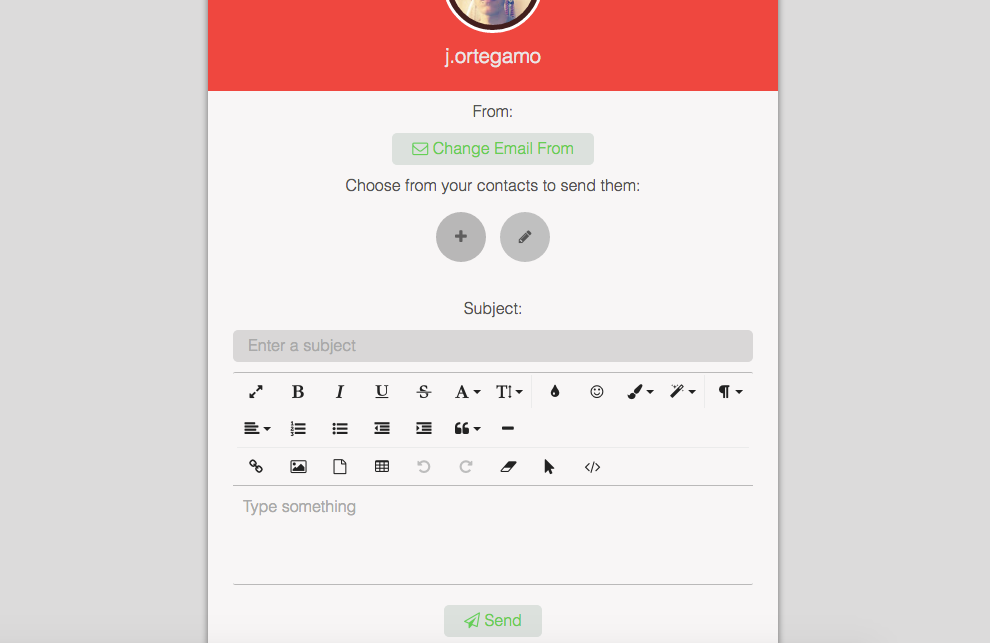
\includegraphics[width=0.8\textwidth]{email-sender-writter.png}
	\caption{P�gina para componer emails}
	\label{fig:email-writter}
\end{figure}




\begin{figure}[htpb]
	\centering
	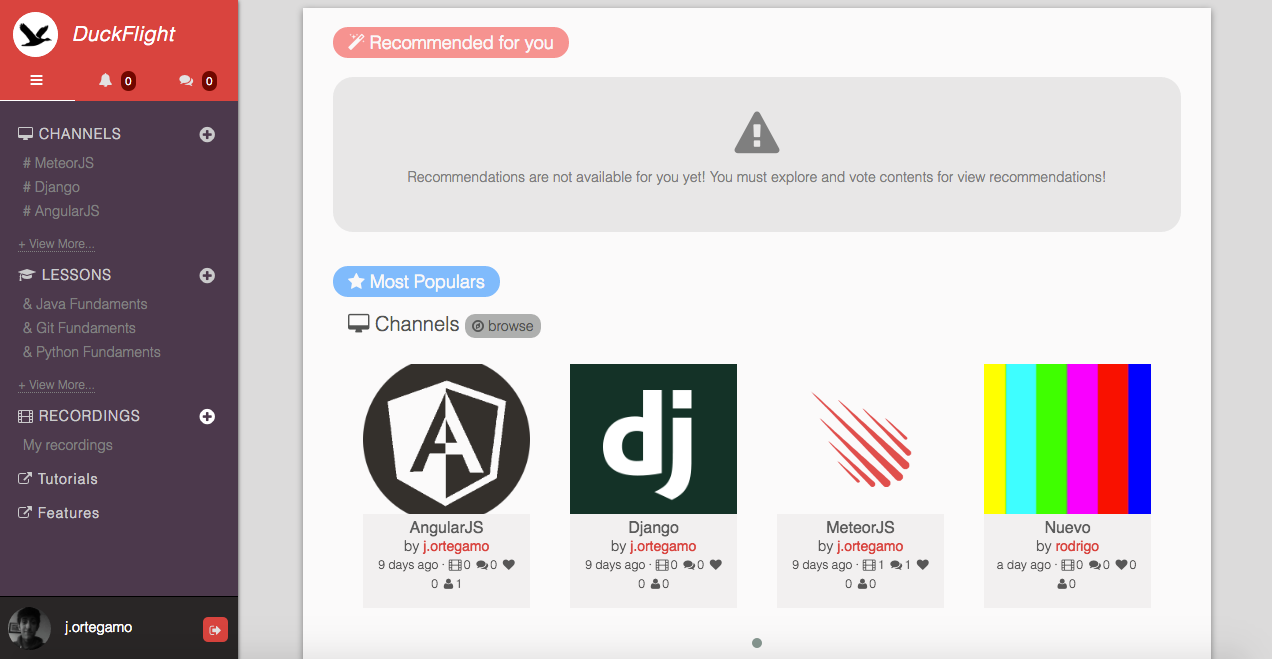
\includegraphics[width=0.8\textwidth]{main-page.png}
	\caption{P�gina principal de la aplicaci�n}
	\label{fig:main-page}
\end{figure}

\begin{figure}[htpb]
	\centering
	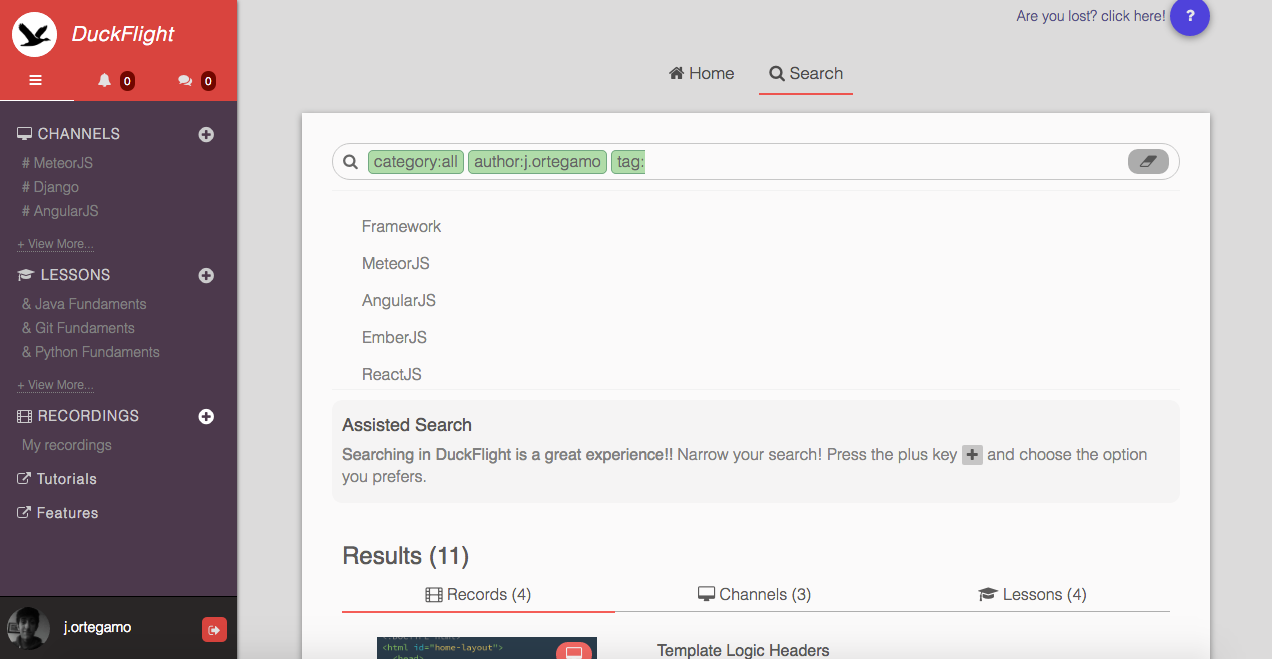
\includegraphics[width=0.8\textwidth]{search.png}
	\caption{Buscador}
	\label{fig:search}
\end{figure}



\begin{figure}[htpb]
	\centering
	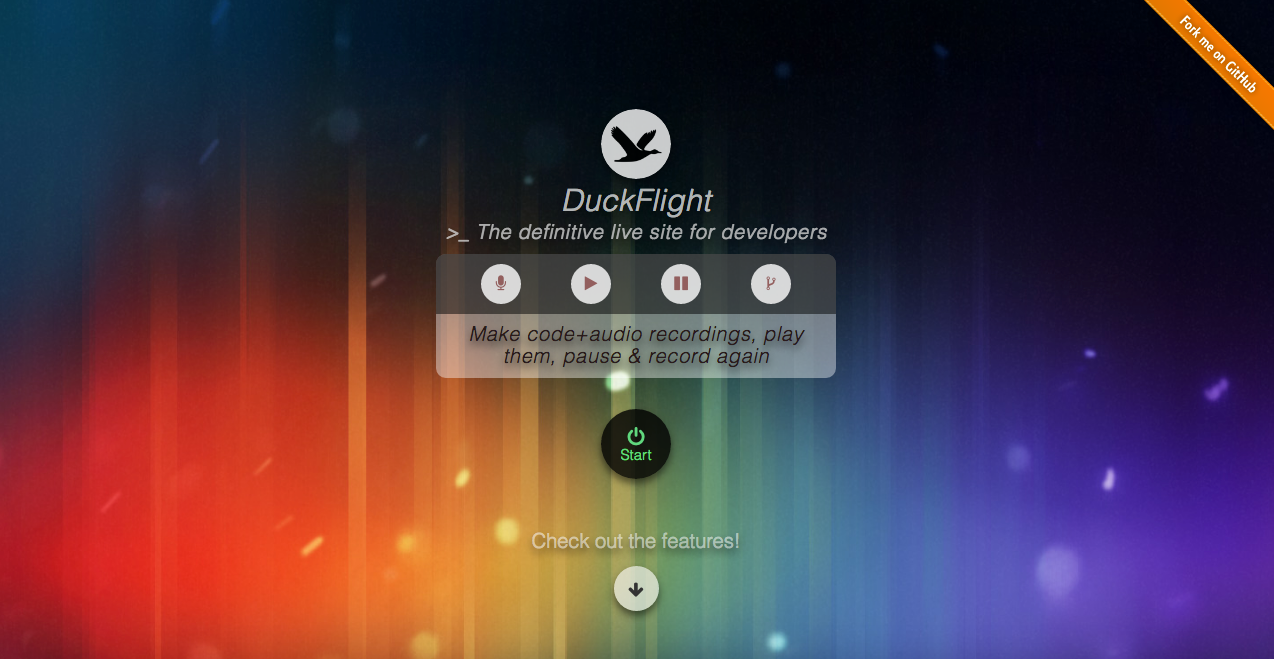
\includegraphics[width=0.8\textwidth]{start-page.png}
	\caption{P�gina de inicio}
	\label{fig:start-page}
\end{figure}

\begin{figure}[htpb]
	\centering
	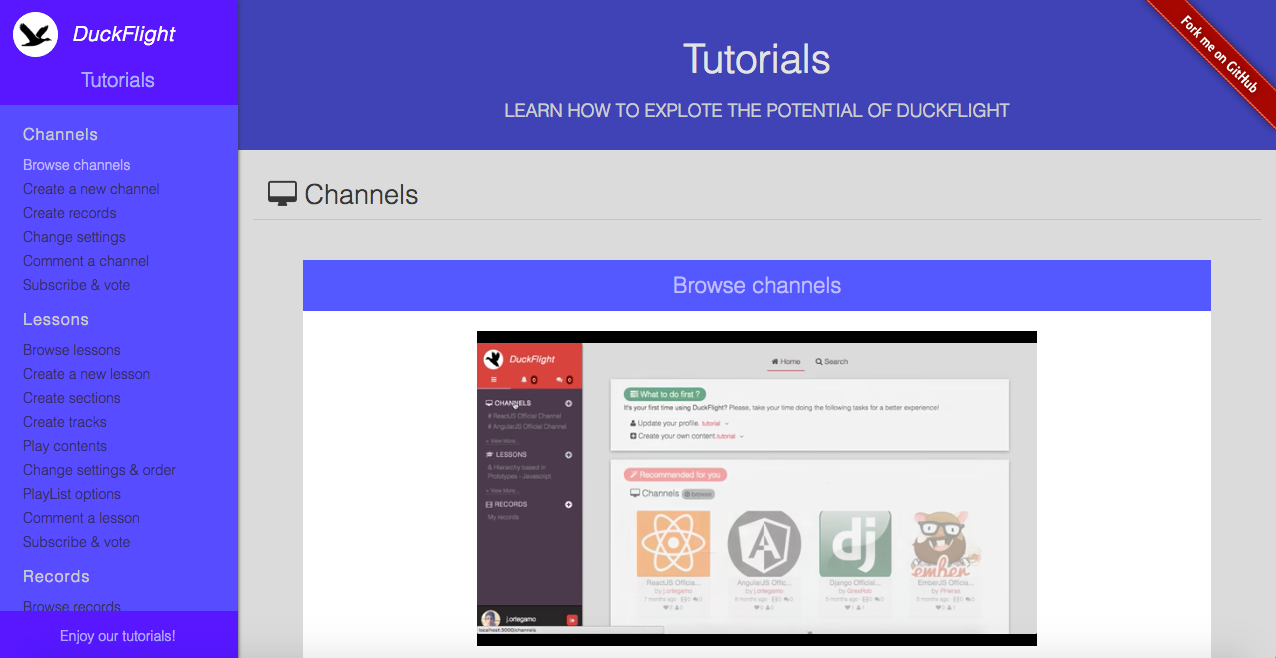
\includegraphics[width=0.8\textwidth]{tutorials.png}
	\caption{Espacio para tutoriales}
	\label{fig:tutorials}
\end{figure}

\begin{figure}[htpb]
	\centering
	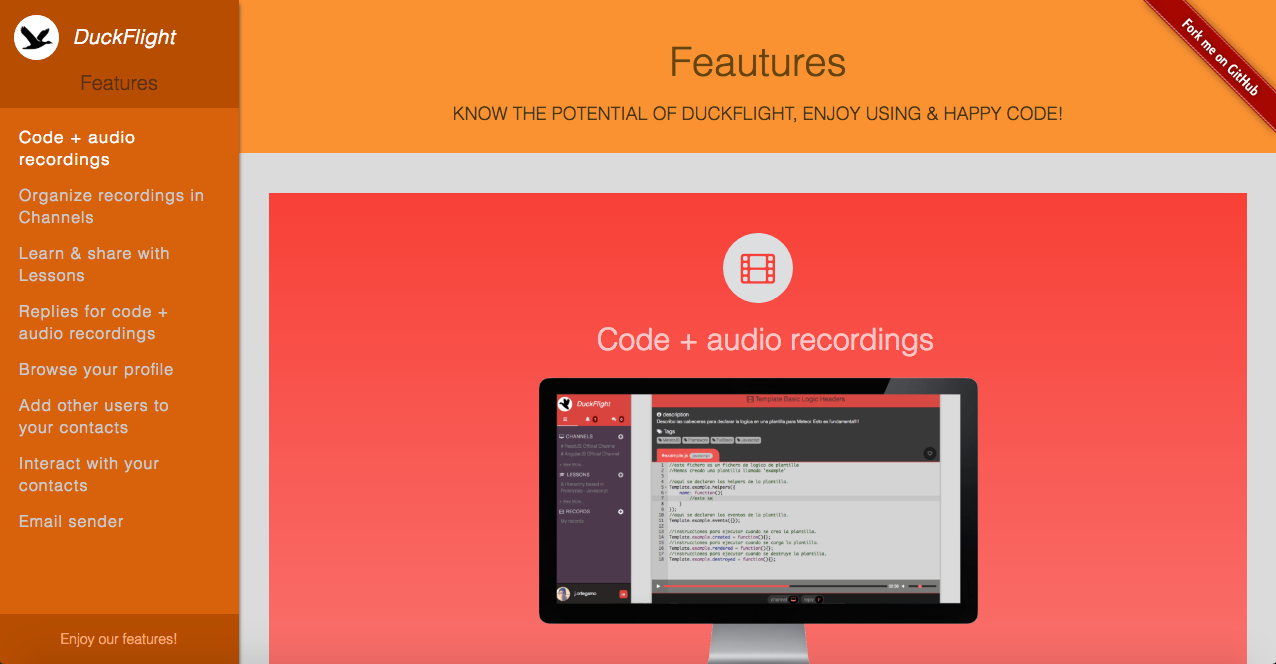
\includegraphics[width=0.8\textwidth]{features.png}
	\caption{Espacio para features}
	\label{fig:features}
\end{figure}



\begin{figure}[htpb]
	\centering
	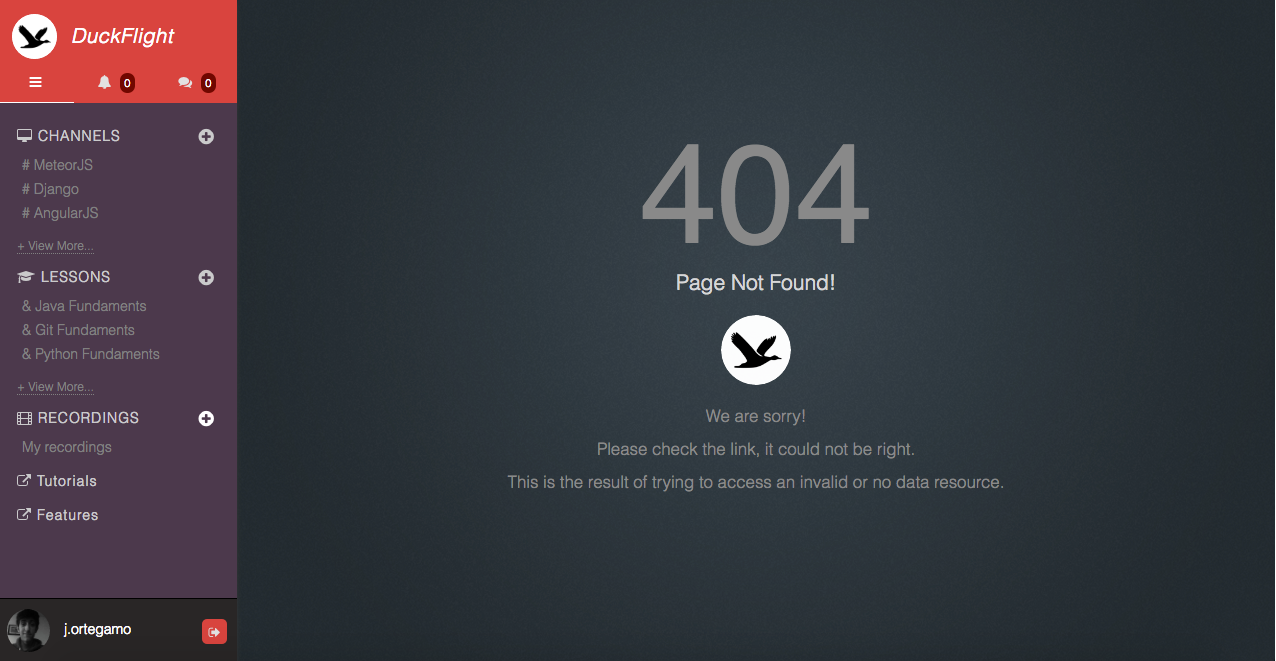
\includegraphics[width=0.8\textwidth]{notFound.png}
	\caption{P�gina 404}
	\label{fig:notFound}
\end{figure}

\begin{figure}[htpb]
	\centering
	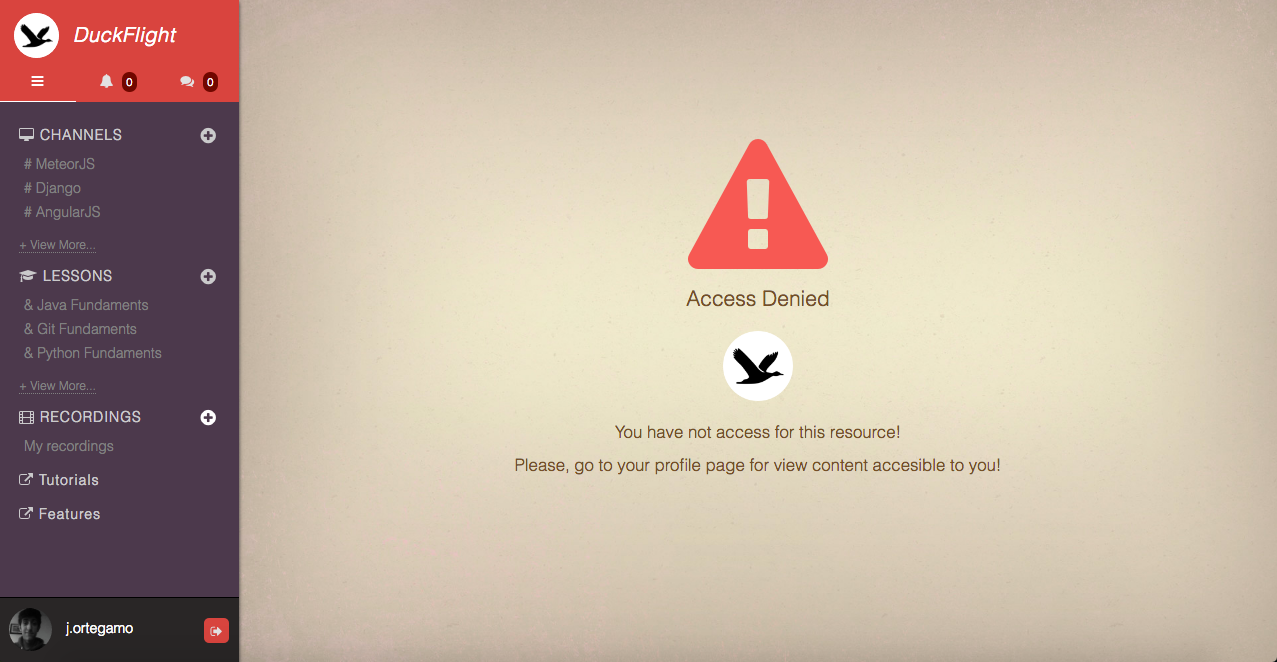
\includegraphics[width=0.8\textwidth]{accessDenied.png}
	\caption{P�gina Acceso Denegado}
	\label{fig:accessDenied}
\end{figure}
